% I compile with latexmk -pdf -interaction=nonstopmode -halt-on-error main.tex.
% I keep the paper's wording, printed precision and claims unchanged.
% I map computed numeric macros to summary.json below; other macros retain fixed source values.
% I keep Figure 1 as a static PDF; changing text macros does not redraw that figure.
\documentclass[10pt,a4paper]{article}
\usepackage[T1]{fontenc}
\usepackage{lmodern}
\usepackage[margin=19mm]{geometry}
\usepackage{amsmath,amssymb,booktabs,array,graphicx,float}
\usepackage[authoryear,round]{natbib}
\usepackage{microtype}
\usepackage{caption}
\usepackage{fancyhdr}
\usepackage[hidelinks]{hyperref}
\captionsetup{font=small,labelsep=period}
\setlength{\parindent}{0pt}
\setlength{\parskip}{6pt}
\setlength{\emergencystretch}{2em}
\setlength{\tabcolsep}{7pt}
\pagestyle{fancy}
\fancyhf{}
\renewcommand{\headrulewidth}{0pt}
\fancyfoot[L]{\footnotesize implied-odds | exploratory historical evidence}
\fancyfoot[R]{\footnotesize\thepage}
\renewcommand{\refname}{References.}
\setlength{\bibsep}{4pt}
% I embed the small BibTeX style to preserve the source reference wording.
\begin{filecontents*}{references-exact.bst}
ENTRY { author title year note } {} {}
FUNCTION {begin.bib}
{ "\begin{thebibliography}{9}" write$ newline$ }
FUNCTION {end.bib}
{ newline$ "\end{thebibliography}" write$ newline$ }
FUNCTION {entry}
{ newline$
  "\bibitem[" write$ author write$ "(" write$
  year empty$ { skip$ } { year write$ } if$
  ")]" write$ "{" write$ cite$ write$ "}" write$ newline$
  author write$
  year empty$ { ", " write$ }
    { " (" write$ year write$ "), " write$ } if$
  title write$ ", " write$ note write$ "." write$ newline$
}
FUNCTION {misc} {entry}
READ
EXECUTE {begin.bib}
ITERATE {entry}
EXECUTE {end.bib}
\end{filecontents*}

% I update each value from the JSON path or fixed-source note immediately above it.
% Fixed wording or parameter in the source paper.
\newcommand{\Unit}{1}
% Fixed wording or parameter in the source paper.
\newcommand{\PowerTwo}{2}
% Fixed wording or parameter in the source paper.
\newcommand{\InterceptIndex}{0}
% $.plan.horizon_hours / 24; format d
\newcommand{\HorizonDays}{30}
% $.plan.horizon_hours; format d
\newcommand{\TargetHours}{720}
% Fixed wording or parameter in the source paper.
\newcommand{\AnnualHours}{8,760}
% AnnualHours without a thousands separator in mathematics.
\newcommand{\AnnualHoursPlain}{8760}
% Fixed wording or parameter in the source paper.
\newcommand{\HoursPerDay}{24}
% Fixed wording or parameter in the source paper.
\newcommand{\DailyDays}{1}
% Fixed wording or parameter in the source paper.
\newcommand{\WeeklyDays}{7}
% $.plan.features_days[2]; format d
\newcommand{\MonthlyDays}{30}
% Fixed wording or parameter in the source paper.
\newcommand{\PercentScale}{100}
% Fixed wording or parameter in the source paper.
\newcommand{\PaperDate}{19 October 2026}
% $.n; format ,d
\newcommand{\MatchedOrigins}{1,357}
% $.plan.historical_origin_start_ms; UTC year
\newcommand{\EvaluationStartYear}{2023}
% $.plan.historical_origin_end_ms; UTC year
\newcommand{\EvaluationEndYear}{2026}
% -$.summary.metrics.qlike_har_dvol_minus_har.mean / $.summary.metrics.qlike_har.mean * 100; format .2f
\newcommand{\MeanLossReductionPercent}{11.35}
% $.summary.metrics.qlike_har_dvol_minus_har.mean; format .5f
\newcommand{\PairedLossMean}{-0.01424}
% Fixed interval level in the source paper.
\newcommand{\ConfidencePercent}{95}
% $.summary.metrics.qlike_har_dvol_minus_har.confidence_interval_95[0]; format .5f
\newcommand{\PairedLossLower}{-0.03490}
% $.summary.metrics.qlike_har_dvol_minus_har.confidence_interval_95[1]; format +.5f
\newcommand{\PairedLossUpper}{+0.00505}
% $.summary.metrics.qlike_har_dvol_minus_har.effective_sample_size; format .2f
\newcommand{\PairedLossEffectiveN}{51.71}
% $.plan.minimum_effective_sample_size; format d
\newcommand{\MinimumEffectiveN}{60}
% Fixed wording or parameter in the source paper.
\newcommand{\SectionA}{1}
% Fixed wording or parameter in the source paper.
\newcommand{\RetainedHourlyCandles}{48,626}
% Fixed wording or parameter in the source paper.
\newcommand{\RetainedDVOLCandles}{1,996}
% Fixed wording or parameter in the source paper.
\newcommand{\DownloadDate}{19 October 2026}
% Fixed wording or parameter in the source paper.
\newcommand{\EvaluationStartDay}{1}
% Fixed wording or parameter in the source paper.
\newcommand{\EvaluationEndDay}{18}
% Fixed wording or parameter in the source paper.
\newcommand{\RequiredCloses}{721}
% $.plan.training_completed_origins; format d
\newcommand{\TrainingLabels}{365}
% $.plan.forecast_floor_variance; source spelling 1e-6
\newcommand{\VarianceFloorText}{1e-6}
% Fixed wording or parameter in the source paper.
\newcommand{\QLIKEUnit}{1}
% $.summary.metrics.qlike_trailing.mean; format .5f
\newcommand{\MeanQLIKETrailing}{0.16670}
% $.summary.metrics.qlike_dvol.mean; format .5f
\newcommand{\MeanQLIKEDvol}{0.09611}
% $.summary.metrics.qlike_har.mean; format .5f
\newcommand{\MeanQLIKEHar}{0.12548}
% $.summary.metrics.qlike_har_dvol.mean; format .5f
\newcommand{\MeanQLIKEHardvol}{0.11123}
% Fixed wording or parameter in the source paper.
\newcommand{\SectionB}{2}
% Fixed wording or parameter in the source paper.
\newcommand{\TailOnePercent}{1}
% Fixed wording or parameter in the source paper.
\newcommand{\TailFivePercent}{5}
% $.concentration.har_dvol.top_absolute_contributions.1.share_absolute_loss_difference * 100; format .1f
\newcommand{\TailOneSharePercent}{8.6}
% $.concentration.har_dvol.top_absolute_contributions.5.share_absolute_loss_difference * 100; format .1f
\newcommand{\TailFiveSharePercent}{27.8}
% $.concentration.har_dvol.leave_one_year_out.2023JSON object key
\newcommand{\LeaveYearAYear}{2023}
% $.concentration.har_dvol.leave_one_year_out.2023.n; format d
\newcommand{\LeaveYearAOrigins}{992}
% $.concentration.har_dvol.leave_one_year_out.2023.mean; format .5f
\newcommand{\LeaveYearAMean}{-0.01233}
% $.concentration.har_dvol.leave_one_year_out.2024JSON object key
\newcommand{\LeaveYearBYear}{2024}
% $.concentration.har_dvol.leave_one_year_out.2024.n; format d
\newcommand{\LeaveYearBOrigins}{991}
% $.concentration.har_dvol.leave_one_year_out.2024.mean; format .5f
\newcommand{\LeaveYearBMean}{-0.01260}
% $.concentration.har_dvol.leave_one_year_out.2025JSON object key
\newcommand{\LeaveYearCYear}{2025}
% $.concentration.har_dvol.leave_one_year_out.2025.n; format d
\newcommand{\LeaveYearCOrigins}{992}
% $.concentration.har_dvol.leave_one_year_out.2025.mean; format .5f
\newcommand{\LeaveYearCMean}{-0.01072}
% $.concentration.har_dvol.leave_one_year_out.2026JSON object key
\newcommand{\LeaveYearDYear}{2026}
% $.concentration.har_dvol.leave_one_year_out.2026.n; format d
\newcommand{\LeaveYearDOrigins}{1096}
% $.concentration.har_dvol.leave_one_year_out.2026.mean; format .5f
\newcommand{\LeaveYearDMean}{-0.02065}
% Fixed wording or parameter in the source paper.
\newcommand{\NonoverlapPhases}{30}
% min($.nonoverlap_phases[*].n); format d
\newcommand{\MinimumPhaseOutcomes}{45}
% max($.nonoverlap_phases[*].n); format d
\newcommand{\MaximumPhaseOutcomes}{46}
% $.plan.decision.annual_volatility_budget; format .2f
\newcommand{\BudgetWeight}{0.20}
% $.plan.decision.annual_volatility_budget squared; format .2f
\newcommand{\BudgetVariance}{0.04}
% $.plan.decision.annual_volatility_budget * 100; format .0f
\newcommand{\BudgetPercent}{20}
% $.decision.trailing.weight; format .3f
\newcommand{\DecisionTrailingWeight}{0.469}
% $.decision.trailing.squared_variance_budget_error; format .7f
\newcommand{\DecisionTrailingBudgetError}{0.0008186}
% $.decision.trailing.budget_exceeded * 100; format .1f
\newcommand{\DecisionTrailingBudgetExceededPercent}{46.7}
% $.decision.dvol.weight; format .3f
\newcommand{\DecisionDvolWeight}{0.418}
% $.decision.dvol.squared_variance_budget_error; format .7f
\newcommand{\DecisionDvolBudgetError}{0.0002872}
% $.decision.dvol.budget_exceeded * 100; format .1f
\newcommand{\DecisionDvolBudgetExceededPercent}{29.6}
% $.decision.har.weight; format .3f
\newcommand{\DecisionHarWeight}{0.420}
% $.decision.har.squared_variance_budget_error; format .7f
\newcommand{\DecisionHarBudgetError}{0.0004014}
% $.decision.har.budget_exceeded * 100; format .1f
\newcommand{\DecisionHarBudgetExceededPercent}{36.3}
% $.decision.har_dvol.weight; format .3f
\newcommand{\DecisionHardvolWeight}{0.437}
% $.decision.har_dvol.squared_variance_budget_error; format .7f
\newcommand{\DecisionHardvolBudgetError}{0.0004196}
% $.decision.har_dvol.budget_exceeded * 100; format .1f
\newcommand{\DecisionHardvolBudgetExceededPercent}{41.7}
% $.summary.metrics.risk_budget_har_dvol_minus_har.mean; format +.7f
\newcommand{\RiskLossMean}{+0.0000182}
% $.summary.metrics.risk_budget_har_dvol_minus_har.confidence_interval_95[0]; format +.7f
\newcommand{\RiskLossLower}{-0.0000818}
% $.summary.metrics.risk_budget_har_dvol_minus_har.confidence_interval_95[1]; format +.7f
\newcommand{\RiskLossUpper}{+0.0001221}
% $.plan.decision.entry_exit_fee_bps[0]; format d
\newcommand{\FeeZeroBps}{0}
% $.plan.decision.entry_exit_fee_bps[1]; format d
\newcommand{\FeeFiveBps}{5}
% $.plan.decision.entry_exit_fee_bps[2]; format d
\newcommand{\FeeTenBps}{10}
% $.plan.decision.entry_exit_fee_bps[3]; format d
\newcommand{\FeeTwentyBps}{20}
% Fixed wording or parameter in the source paper.
\newcommand{\SectionC}{3}
% $.plan.bootstrap_resamples; format ,d
\newcommand{\BootstrapDraws}{5,000}
% $.plan.expected_block_days; format d
\newcommand{\ExpectedBlockDays}{60}
% $.plan.hac_lags_days; format d
\newcommand{\HACLags}{59}
% $.plan.sensitivity_block_days[0]; format d
\newcommand{\SensitivityThirtyDays}{30}
% $.plan.sensitivity_block_days[1]; format d
\newcommand{\SensitivityNinetyDays}{90}
% $.plan.sensitivity_block_days[2]; format d
\newcommand{\SensitivityOneEightyDays}{180}
% $.plan.sensitivity_block_days[3]; format d
\newcommand{\SensitivityYearDays}{365}
% $.plan.simulation.replications; format d
\newcommand{\SimulationReplications}{200}
% $.plan.simulation.sample_sizes[0]; format d
\newcommand{\SimulationShortN}{365}
% $.plan.simulation.sample_sizes[1]; format ,d
\newcommand{\SimulationLongNGrouped}{1,357}
% $.plan.simulation.bootstrap_resamples; format ,d
\newcommand{\SimulationBootstrapDraws}{2,000}
% Fixed wording or parameter in the source paper.
\newcommand{\NegativeUnit}{-1}
% Fixed wording or parameter in the source paper.
\newcommand{\PersistenceDays}{365}
% $.plan.simulation.power_mean_shifts[1]; format .2f
\newcommand{\AlternativeShift}{-0.25}
% $.inference_simulations.rows[0].n; format d
\newcommand{\NullScenarioAN}{365}
% $.inference_simulations.rows[0].ungated_rejection_rate * 100; format .1f
\newcommand{\NullScenarioARejectionPercent}{19.0}
% $.inference_simulations.rows[0].ungated_mc_interval_95[0] * 100; format .1f
\newcommand{\NullScenarioALowerPercent}{14.2}
% $.inference_simulations.rows[0].ungated_mc_interval_95[1] * 100; format .1f
\newcommand{\NullScenarioAUpperPercent}{25.0}
% $.inference_simulations.rows[0].gate_pass_rate * 100; format .1f
\newcommand{\NullScenarioAGatePercent}{0.0}
% $.inference_simulations.rows[2].n; format d
\newcommand{\NullScenarioBN}{365}
% $.inference_simulations.rows[2].ungated_rejection_rate * 100; format .1f
\newcommand{\NullScenarioBRejectionPercent}{49.0}
% $.inference_simulations.rows[2].ungated_mc_interval_95[0] * 100; format .1f
\newcommand{\NullScenarioBLowerPercent}{42.2}
% $.inference_simulations.rows[2].ungated_mc_interval_95[1] * 100; format .1f
\newcommand{\NullScenarioBUpperPercent}{55.9}
% $.inference_simulations.rows[2].gate_pass_rate * 100; format .1f
\newcommand{\NullScenarioBGatePercent}{0.0}
% $.inference_simulations.rows[4].n; format d
\newcommand{\NullScenarioCN}{365}
% $.inference_simulations.rows[4].ungated_rejection_rate * 100; format .1f
\newcommand{\NullScenarioCRejectionPercent}{16.0}
% $.inference_simulations.rows[4].ungated_mc_interval_95[0] * 100; format .1f
\newcommand{\NullScenarioCLowerPercent}{11.6}
% $.inference_simulations.rows[4].ungated_mc_interval_95[1] * 100; format .1f
\newcommand{\NullScenarioCUpperPercent}{21.7}
% $.inference_simulations.rows[4].gate_pass_rate * 100; format .1f
\newcommand{\NullScenarioCGatePercent}{0.0}
% $.inference_simulations.rows[6].n; format d
\newcommand{\NullScenarioDN}{1357}
% $.inference_simulations.rows[6].ungated_rejection_rate * 100; format .1f
\newcommand{\NullScenarioDRejectionPercent}{10.0}
% $.inference_simulations.rows[6].ungated_mc_interval_95[0] * 100; format .1f
\newcommand{\NullScenarioDLowerPercent}{6.6}
% $.inference_simulations.rows[6].ungated_mc_interval_95[1] * 100; format .1f
\newcommand{\NullScenarioDUpperPercent}{14.9}
% $.inference_simulations.rows[6].gate_pass_rate * 100; format .1f
\newcommand{\NullScenarioDGatePercent}{1.5}
% $.inference_simulations.rows[8].n; format d
\newcommand{\NullScenarioEN}{1357}
% $.inference_simulations.rows[8].ungated_rejection_rate * 100; format .1f
\newcommand{\NullScenarioERejectionPercent}{45.0}
% $.inference_simulations.rows[8].ungated_mc_interval_95[0] * 100; format .1f
\newcommand{\NullScenarioELowerPercent}{38.3}
% $.inference_simulations.rows[8].ungated_mc_interval_95[1] * 100; format .1f
\newcommand{\NullScenarioEUpperPercent}{51.9}
% $.inference_simulations.rows[8].gate_pass_rate * 100; format .1f
\newcommand{\NullScenarioEGatePercent}{0.0}
% $.inference_simulations.rows[10].n; format d
\newcommand{\NullScenarioFN}{1357}
% $.inference_simulations.rows[10].ungated_rejection_rate * 100; format .1f
\newcommand{\NullScenarioFRejectionPercent}{8.5}
% $.inference_simulations.rows[10].ungated_mc_interval_95[0] * 100; format .1f
\newcommand{\NullScenarioFLowerPercent}{5.4}
% $.inference_simulations.rows[10].ungated_mc_interval_95[1] * 100; format .1f
\newcommand{\NullScenarioFUpperPercent}{13.2}
% $.inference_simulations.rows[10].gate_pass_rate * 100; format .1f
\newcommand{\NullScenarioFGatePercent}{1.5}
% min(one-year null $.inference_simulations.rows[*].ungated_rejection_rate) * 100; format .0f
\newcommand{\ShortNullMinimumRejectionPercent}{16}
% max(one-year null $.inference_simulations.rows[*].ungated_rejection_rate) * 100; format .0f
\newcommand{\ShortNullMaximumRejectionPercent}{49}
% Fixed wording or parameter in the source paper.
\newcommand{\NominalRejectionPercent}{5}
% One-year null/alternative Wilson 95 percent upper bound at zero passes out of 200; format .1f percent
\newcommand{\GatePassUpperPercent}{1.9}
% Fixed wording or parameter in the source paper.
\newcommand{\SectionD}{4}
% $.plan.future.n_planned_origins; format d
\newcommand{\PlannedOrigins}{365}
% $.plan.future.origin_start_ms; UTC date
\newcommand{\HARStartDate}{21 October 2026}
% $.plan.future.origin_end_ms; UTC date
\newcommand{\HAREndDate}{20 October 2027}
% $.plan.future; fixed UTC clock from the source paper.
\newcommand{\HAROriginTime}{01:00}
% $.plan.future; fixed UTC clock from the source paper.
\newcommand{\HARFreezeStartTime}{00:10}
% $.plan.future; fixed UTC clock from the source paper.
\newcommand{\HARFreezeEndTime}{00:50}
% $.plan.future.origin_end_ms plus horizon_hours; UTC date
\newcommand{\HARMaturityDate}{19 November 2027}
% $.plan.future.analysis_at_ms; UTC date
\newcommand{\HARAnalysisDate}{21 November 2027}
% Fixed wording or parameter in the source paper.
\newcommand{\SVICutoffDate}{20 October 2027}
% Fixed wording or parameter in the source paper.
\newcommand{\SVITime}{08:00}
% Fixed wording or parameter in the source paper.
\newcommand{\SVIAnalysisDate}{22 October 2027}
% Fixed wording or parameter in the source paper.
\newcommand{\PythonVersion}{3.12}
% Fixed wording or parameter in the source paper.
\newcommand{\FigureNumber}{1}
% Source bibliography.
\newcommand{\CorsiYear}{2009}
% Source bibliography.
\newcommand{\PattonYear}{2011}
% Source bibliography.
\newcommand{\BootstrapYear}{1994}
% Source bibliography; identifier.
\newcommand{\CorsiDOI}{10.1093/jjfinec/nbp001}
% Source bibliography; identifier.
\newcommand{\PattonDOI}{10.1016/j.jeconom.2010.03.034}
% Source bibliography; identifier.
\newcommand{\BootstrapDOI}{10.1080/01621459.1994.10476870}
\renewcommand{\thefigure}{\FigureNumber}

\begin{document}

\begin{center}{\LARGE\bfseries Does DVOL add information beyond HAR?\par}\end{center}

\begin{center}\small A retrospective BTC variance forecast study | 50kfunded | \PaperDate{}\end{center}

\textbf{Abstract.} I compare direct \HorizonDays{}-day HAR forecasts with the same regression augmented by BTC DVOL, using \MatchedOrigins{} matched daily origins from \EvaluationStartYear{} to \EvaluationEndYear{}. Augmentation lowers mean QLIKE by \MeanLossReductionPercent{}\%, but its paired difference is \PairedLossMean{}, with descriptive \ConfidencePercent{}\% interval [\PairedLossLower{}, \PairedLossUpper{}] and estimated ESS \PairedLossEffectiveN{}, below the fixed threshold of \MinimumEffectiveN{}. I find no clear improvement in a fixed variance-budget decision. My inference stress tests also show that one year of overlapping daily forecasts has no demonstrated useful confirmatory power under the declared gate, so I lock the future study as evidence collection and keep formal superiority claims disabled.

\begin{figure}[H]
\centering
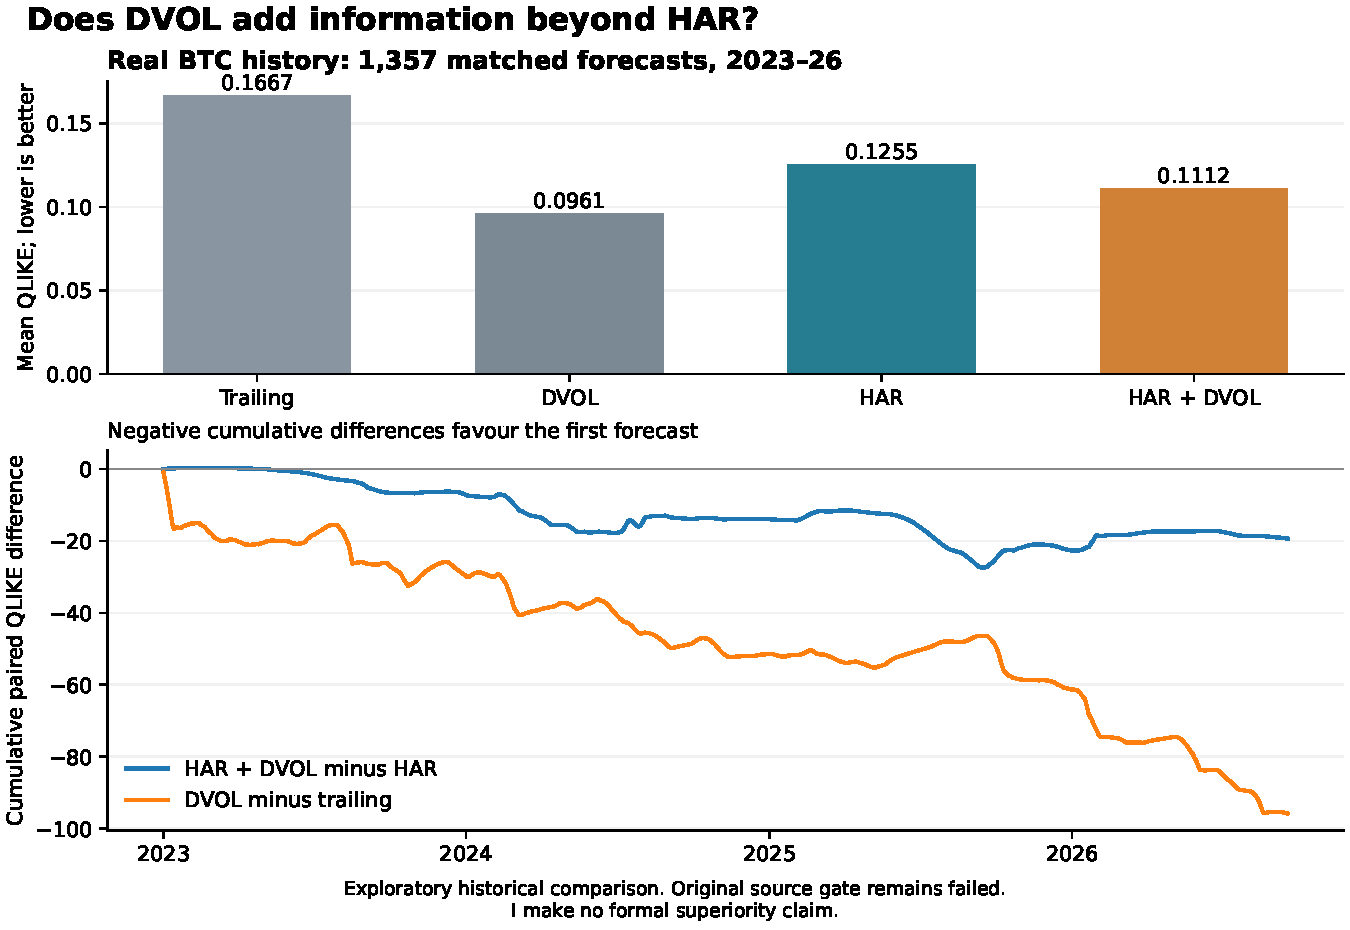
\includegraphics[width=\linewidth]{figure-1.pdf}
\caption{I use real retained historical inputs. Both panels use the same \MatchedOrigins{} origins. The lower panel shows error accumulation, rather than trading profit. All historical findings remain exploratory; the original vendor all-OHLC validation gate remains failed.}
\label{fig:headline}
\end{figure}

\clearpage

\section*{\SectionA{}. Question, inputs and matched design}

I ask whether option-implied variance adds forecasting information beyond daily, weekly and monthly realised-variance components. I use Corsi's HAR construction as a parsimonious price-history benchmark, adapted to a direct \HorizonDays{}-day target. I compare the benchmark with the same model plus previous completed daily DVOL variance. I also retain raw DVOL and trailing variance.

I downloaded \RetainedHourlyCandles{} hourly BTC-PERPETUAL candles and \RetainedDVOLCandles{} daily BTC DVOL candles on \DownloadDate{}. My matched evaluation uses daily midnight origins from \EvaluationStartDay{} January \EvaluationStartYear{} through \EvaluationEndDay{} September \EvaluationEndYear{}. I use the next \TargetHours{} hourly log-return squares, annualised by \AnnualHours{}, as the target. Each \TargetHours{}-return window requires \RequiredCloses{} completed closes. Historical downloads do not establish original unrevised vintages.

At each origin I fit both regressions using exactly the latest \TrainingLabels{} labels whose full \HorizonDays{}-day targets have ended. My HAR features are prior \DailyDays{}-, \WeeklyDays{}- and \MonthlyDays{}-day annualised variances; the augmented model adds squared DVOL/\PercentScale{}. I use level OLS with an intercept. I centre and scale features using the training rows only. I fix a \VarianceFloorText{} annual-variance floor, retain raw predictions, and count every floor hit. Neither model hits it in this sample.


\begin{align*}
V_t^{(\HorizonDays{}\mathrm{d})} &= \frac{\AnnualHoursPlain{}}{\TargetHours{}}
  \sum_{h=\Unit{}}^{\TargetHours{}} r_{t+h}^{\PowerTwo{}},\\
RV_t^{(k)} &= \frac{\AnnualHoursPlain{}}{\HoursPerDay{}\,k}
  \sum_{h=\Unit{}}^{\HoursPerDay{}\,k}r_{t-h+\Unit{}}^{\PowerTwo{}},
\quad k\in\{\DailyDays{},\WeeklyDays{},\MonthlyDays{}\},\\
\widehat V^{(\HorizonDays{}\mathrm{d}),\mathrm{HAR}}_t
 &= \widehat\beta_{\InterceptIndex{},t}
  +\widehat\beta_{d,t}RV_t^{(\DailyDays{})}
  +\widehat\beta_{w,t}RV_t^{(\WeeklyDays{})}
  +\widehat\beta_{m,t}RV_t^{(\MonthlyDays{})},\\
\widehat V^{(\HorizonDays{}\mathrm{d}),\mathrm{HAR+DVOL}}_t
 &= \widehat\gamma_{\InterceptIndex{},t}
  +\widehat\gamma_{d,t}RV_t^{(\DailyDays{})}
  +\widehat\gamma_{w,t}RV_t^{(\WeeklyDays{})}
  +\widehat\gamma_{m,t}RV_t^{(\MonthlyDays{})}
  +\widehat\gamma_{D,t}
    \left(\frac{\mathrm{DVOL}^{\mathrm{prev.close}}_t}{\PercentScale{}}\right)^{\PowerTwo{}}.
\end{align*}


I score
\[
\operatorname{QLIKE}
 =\frac{\text{realised}}{\text{forecast}}
  -\log\!\left(\frac{\text{realised}}{\text{forecast}}\right)
  -\QLIKEUnit{}.
\]
I compute every comparison on identical origins. The additional historical work follows inspection of these data, so chronological training does not make this an untouched experiment.

\begin{center}
\small
\begin{tabular}{lrl}
\toprule
Forecast & Mean QLIKE & Role \\
\midrule
Trailing \HorizonDays{}-day & \MeanQLIKETrailing{} & Reference \\
Raw DVOL & \MeanQLIKEDvol{} & Reference \\
HAR & \MeanQLIKEHar{} & Benchmark \\
HAR + DVOL & \MeanQLIKEHardvol{} & Augmentation \\
\bottomrule
\end{tabular}
\end{center}

I estimate an augmentation difference of \PairedLossMean{}, with interval [\PairedLossLower{}, \PairedLossUpper{}]. The interval includes zero and the ESS gate fails. Raw DVOL has the lowest point loss, which also exposes estimation risk in the fitted augmentation.

I include level Mincer-Zarnowitz regressions with HAC uncertainty, a joint HAR calibration/encompassing restriction, and a separate incremental-coefficient restriction with the HAR slope and intercept unrestricted. These generated-forecast diagnostics are exploratory; I do not treat their p-values as additional primary discoveries. Coefficients and uncertainty are in summary.json.

\clearpage

\section*{\SectionB{}. Loss concentration and a concrete decision}

I find that the largest \TailOnePercent{}\% and \TailFivePercent{}\% of absolute augmentation loss differences account for \TailOneSharePercent{}\% and \TailFiveSharePercent{}\% of total absolute differences. Their signed contributions are positive, so these largest observations hurt augmentation. The overall mean is still negative. This does not support a simple story that augmentation wins only by avoiding the most extreme losses.

\begin{center}
\small
\begin{tabular}{lrr}
\toprule
Year left out & Remaining origins & Mean augmentation difference \\
\midrule
\LeaveYearAYear{} & \LeaveYearAOrigins{} & \LeaveYearAMean{} \\
\LeaveYearBYear{} & \LeaveYearBOrigins{} & \LeaveYearBMean{} \\
\LeaveYearCYear{} & \LeaveYearCOrigins{} & \LeaveYearCMean{} \\
\LeaveYearDYear{} & \LeaveYearDOrigins{} & \LeaveYearDMean{} \\
\bottomrule
\end{tabular}
\end{center}

I retain contributions for every fixed calendar quarter, extreme-origin dates, and all \NonoverlapPhases{} non-overlapping starting phases. The phase samples contain only \MinimumPhaseOutcomes{} or \MaximumPhaseOutcomes{} outcomes and are dependent. I use these displays to expose concentration, not to select a favourable crisis window or claim an ex-ante regime rule.

For decision relevance I fix an illustrative annual volatility budget of \BudgetPercent{}\% and weight 
\[
w=\min\!\left(\Unit{},\frac{\BudgetWeight{}}{\sqrt{\text{forecast variance}}}\right).
\]
I measure the squared error
\[
\left(w^{\PowerTwo{}}\times\text{realised variance}-\BudgetVariance{}\right)^{\PowerTwo{}}.
\]
This assumes constant fractional exposure for the variance calculation. I do not implement a fixed-unit portfolio, rebalancing, funding or profit, and this rule is not claimed optimal for squared budget error.

\begin{center}
\small
\begin{tabular}{lrrl}
\toprule
Forecast & Mean weight & \shortstack{Mean squared\\budget error} & Budget exceeded \\
\midrule
Trailing & \DecisionTrailingWeight{} & \DecisionTrailingBudgetError{} & \DecisionTrailingBudgetExceededPercent{}\% \\
DVOL & \DecisionDvolWeight{} & \DecisionDvolBudgetError{} & \DecisionDvolBudgetExceededPercent{}\% \\
HAR & \DecisionHarWeight{} & \DecisionHarBudgetError{} & \DecisionHarBudgetExceededPercent{}\% \\
HAR + DVOL & \DecisionHardvolWeight{} & \DecisionHardvolBudgetError{} & \DecisionHardvolBudgetExceededPercent{}\% \\
\bottomrule
\end{tabular}
\end{center}

I get augmented-minus-HAR risk loss \RiskLossMean{}, with interval [\RiskLossLower{}, \RiskLossUpper{}]. Lower mean QLIKE does not establish a better decision under this loss. I report entry-plus-exit fee amounts separately at \FeeZeroBps{}, \FeeFiveBps{}, \FeeTenBps{} and \FeeTwentyBps{} basis points per side; I do not subtract costs from a risk error or infer trading returns.

\clearpage

\section*{\SectionC{}. Dependence and finite-sample inference}

I use \BootstrapDraws{} paired stationary-bootstrap draws with a fixed seed, \ExpectedBlockDays{}-day expected blocks and a \HACLags{}-lag HAC check. I retain \SensitivityThirtyDays{}-, \SensitivityNinetyDays{}-, \SensitivityOneEightyDays{}- and \SensitivityYearDays{}-day block sensitivities. The overlapping targets and rolling fits can create dependence beyond the \SensitivityThirtyDays{}-day target horizon. ESS is a diagnostic estimate, not an observed number of independent episodes.

I simulate \SimulationReplications{} independent samples per declared scenario at n=\SimulationShortN{} and n=\SimulationLongNGrouped{}, using \SimulationBootstrapDraws{} bootstrap draws each. My population null is exactly mean zero without centring each realised sample. I use a \HorizonDays{}-day moving-average loss component, a stationary slow component with persistence exp(\NegativeUnit{}/\PersistenceDays{}), and symmetric rare shocks spread across overlapping windows. The synthetic alternative is a \AlternativeShift{} marginal-standard-deviation shift, not \AlternativeShift{} QLIKE. These stress tests approximate loss dependence and do not simulate the entire rolling HAR estimation pipeline.

\begin{center}
\small
\begin{tabular}{lrrr}
\toprule
n / synthetic process & Ungated rejection & \ConfidencePercent{}\% MC interval & ESS gate passes \\
\midrule
\NullScenarioAN{} / Overlap & \NullScenarioARejectionPercent{}\% & \NullScenarioALowerPercent{}\% to \NullScenarioAUpperPercent{}\% & \NullScenarioAGatePercent{}\% \\
\NullScenarioBN{} / Overlap + slow & \NullScenarioBRejectionPercent{}\% & \NullScenarioBLowerPercent{}\% to \NullScenarioBUpperPercent{}\% & \NullScenarioBGatePercent{}\% \\
\NullScenarioCN{} / Overlap + tails & \NullScenarioCRejectionPercent{}\% & \NullScenarioCLowerPercent{}\% to \NullScenarioCUpperPercent{}\% & \NullScenarioCGatePercent{}\% \\
\NullScenarioDN{} / Overlap & \NullScenarioDRejectionPercent{}\% & \NullScenarioDLowerPercent{}\% to \NullScenarioDUpperPercent{}\% & \NullScenarioDGatePercent{}\% \\
\NullScenarioEN{} / Overlap + slow & \NullScenarioERejectionPercent{}\% & \NullScenarioELowerPercent{}\% to \NullScenarioEUpperPercent{}\% & \NullScenarioEGatePercent{}\% \\
\NullScenarioFN{} / Overlap + tails & \NullScenarioFRejectionPercent{}\% & \NullScenarioFLowerPercent{}\% to \NullScenarioFUpperPercent{}\% & \NullScenarioFGatePercent{}\% \\
\bottomrule
\end{tabular}
\end{center}

At n=\SimulationShortN{} I observe ungated null rejection rates of \ShortNullMinimumRejectionPercent{}\% to \ShortNullMaximumRejectionPercent{}\%, rather than nominal \NominalRejectionPercent{}\%. The ESS gate passes zero of \SimulationReplications{} replications under every one-year null and alternative, giving a Wilson \ConfidencePercent{}\% upper bound around \GatePassUpperPercent{}\% for the pass probability. I therefore have no demonstrated useful confirmatory power for the planned year. At n=\MatchedOrigins{}, conditional estimates sometimes use only one to four passing replications; I retain their wide Monte Carlo intervals.

I committed a separate inference-validation amendment that disables formal superiority claims for the new HAR period. I preserve its fixed terminal date and primary contrast, collect timestamped evidence, and accept an inconclusive terminal result. A later inference design needs its own prospective declaration; I will not change this cohort to recover significance.

\clearpage

\section*{\SectionD{}. Prospective collection, limits and reproduction}

I locked \PlannedOrigins{} future HAR origins from \HARStartDate{} through \HAREndDate{}, each at \HAROriginTime{} UTC. Features end at midnight; I freeze between \HARFreezeStartTime{} and \HARFreezeEndTime{}, then start the outcome at \HAROriginTime{}. I train on the correspondingly shifted historical \HorizonDays{}-day targets completed by midnight. This differs from the midnight target alignment in the retrospective comparison. Final maturity is \HARMaturityDate{}; I fix the terminal analysis at \HARAnalysisDate{}, \HAROriginTime{} UTC.

I require a matching hourly and daily DVOL close for each new forecast, preserve raw capture segments, attach code and input hashes, and check fitting and durable-write completion against the freeze deadline. I count missed scheduled days and do not backfill. I withhold terminal intervals unless all \PlannedOrigins{} planned pairs and source checks exist; late-arriving scores after the fixed analysis cutoff stay excluded.

My separate SVI study still has zero settled research forecasts. Its original protocol and baseline locks remain unchanged. A versioned amendment fixes its expiry cutoff at \SVICutoffDate{}, \SVITime{} UTC and final decision at \SVIAnalysisDate{}, \SVITime{} UTC. Both reporting and CLI inference keep earlier output descriptive and pin terminal data availability. I retain calendar-grid and extrapolated-tail limitations. Local forecast hash chains are not independent public timestamps.

My collector retries recoverable delivery pagination in fresh segments and keeps conflicting immutable prices fatal. I cache cleaning by input, protocol, code and runtime fingerprints, and render reports outside the forecast loop. I publish counts, rejection reasons, local hashes and heartbeat age. A fresh heartbeat does not prove process health. Continuous collection needs an awake online host; short validation recordings do not establish sustained operation.

The original all-OHLC audit remains failed because one unused DVOL open differs. All three audited DVOL closes match, but these dates do not validate the entire history. I use perpetual returns as an index proxy, a single asset and venue, retrieved vintages and overlapping outcomes. I do not identify a causal variance premium or executable edge.

\textbf{Reproduction.} I use Python \PythonVersion{} with requirements-research.txt, then run \newline\textbf{python scripts/build\_research.py}. I retain the full report, matched forecasts, coefficients, training cutoffs, diagnostics, simulation rates and plan hashes. The command reads the checked-in public recordings and makes no market requests.

\begingroup\raggedright

\nocite{corsi,patton,politisromano,deribit}

\bibliographystyle{references-exact}

\bibliography{references}

\endgroup

\end{document}
